\documentclass{article}
\usepackage[utf8]{inputenc}
%allow simultaneous greek and english input
\usepackage[greek,english]{babel}
\usepackage{alphabeta}
%package needed for image template
\usepackage{eso-pic}
%colour links, hrefs, etc whatever colour you like
%use only if needed. Shows warnings on Greek characters but nothing bad actually happens.
%just annoys you

\usepackage[colorlinks = true,
            linkcolor = black,
            urlcolor  = black,
            citecolor = blue,
            anchorcolor = blue]{hyperref}

%create a macro named BackgroundPic for setting a background on the first page
\newcommand\BackgroundPic{
    \put(-3,0){
    \parbox[b][\paperheight]{\paperwidth}{%
    \vfill
    \centering
    
\includegraphics[width=\paperwidth,height=\paperheight]{LATEX_TEMPLATE_V2.pdf}
    \vfill
    }}}
%Info
\title{\vspace{0.2cm}\textbf{Spin and Spintronics: Spin-based Transistors}}
\date{\textbf{23 February\\ v2.0\\[5pt] Nanotechnology Course Project}}
    \author{\textbf{Bantis, Michailidou, Stergiopoulos}}
%include page geometry packages
\usepackage{natbib}
\usepackage{graphicx}
\usepackage[a4paper, total={6.5in, 8in}]{geometry}
%document starts here, who would have imagined that?
\begin{document}
%set AERONAUTICS_REPORT_TEMPLATE as template JUST for this page
%the asterisk means it will be set just for this page
\AddToShipoutPicture*{\BackgroundPic}
 \maketitle
\maketitle
%leave a bunch of empty space for the contents
\vspace{2.8cm}
%shows contents automatically. Every section, subsection, etc automatically shows up here
\tableofcontents{}
%change page
\pagebreak
%create new command about pics on all other pages
\ClearShipoutPicture
\newcommand\Bgpic{
    \put(-4,0){
    \parbox[b][\paperheight]{\paperwidth}{%
    \vfill
    \centering
    
\includegraphics[width=\paperwidth,height=\paperheight]{LATEX_TEMPLATE_V2.pdf}
    \vfill
    }}}
%set background picture for every page after page 2, including page 2
%see, no asterisk
\AddToShipoutPicture{\Bgpic}
%yay, our first section, who would have thought


\section{Standard Model}
\large
\subsection{Overview}
The Standard Model of particle physics currently is humanity’s best and most complete description of the “building blocks” of the universe. It describes three out of the four known fundamental forces in the universe (the electromagnetic force, the weak nuclear force, and the strong nuclear force, but not the gravitational force), and all of the currently known fundamental particles. The Model categorises particles and their respective anti-particles into certain sub-groups (fermions/bosons, quarks/leptons, gauge/scalar bosons) depending on their properties.[1]

\begin{center}
    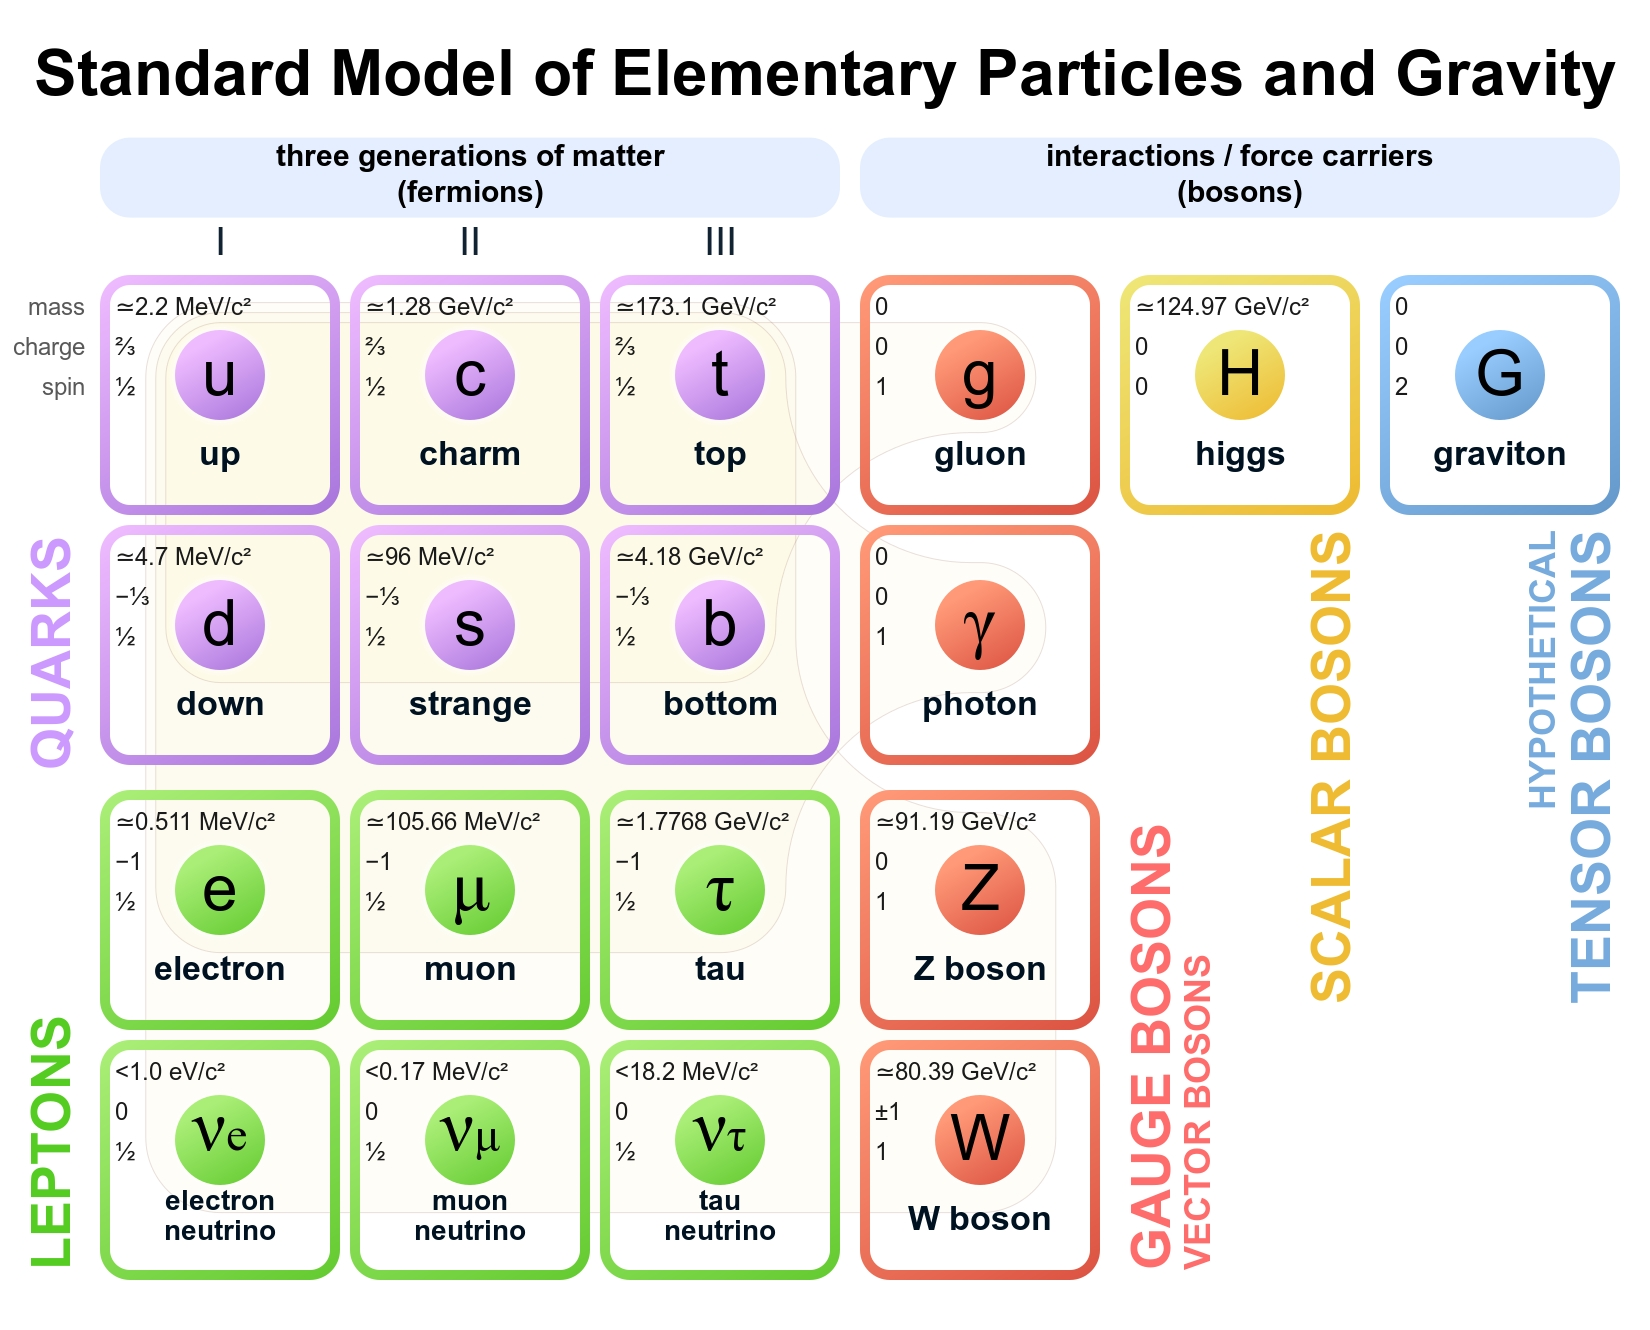
\includegraphics[scale=0.16]{partic.jpg}
\end{center}

\subsection{Fermions}
Fermions are particles with a half-integer spin. The “Fermion” sub-group includes 24 particles in total: 12 particles and their corresponding anti-particles. The only difference between a “normal” particle and an anti-particle is that the latter has a charge opposite to the charge of the former. Fermions obey the Fermi-Dirac statistics and the Pauli exclusion principle. This means that fermionic systems can be described and analysed in terms of one-particle energy states and that any two fermions are unable to occupy the same state in a system.[2][3]. The Fermi-Dirac distribution of identical fermions over energy is described by the equation ${\displaystyle {\bar {\mathcal {N}}}(\varepsilon )={\frac {g(\varepsilon )}{e^{(\varepsilon -\mu )/k_{\rm {B}}T}+1}}}$ (and its special cases), where $\varepsilon$: energy, $\mu$: total chemical potential, $k_{\rm {B}}$: Boltzmann’s constant, and T: absolute temperature.[4]
\pagebreak

\subsection{Bosons}
Bosons are particles with an integer spin. The “Boson” sub-group includes the gluon, the photon, the W+ and W- bosons, the Z boson, the Higgs boson, and the hypothetical graviton. Bosons obey the Bose-Einstein statistics and, unlike fermions, they do not obey the Pauli exclusion principle. This means that an unlimited number of bosons can occupy the same energy state. The theoretical number of bosons in an energy state is described by the equation ${\displaystyle {\bar {n}}_{i}={\frac {g_{i}}{e^{(\varepsilon _{i}-\mu ) / k_{\text{B}}T} - 1}}}$, with $\varepsilon _{i} > \mu$, where $\varepsilon _{i}$ the energy of the state i, and where $g_{i}$: degeneracy of the energy level i.[5]

\section{Spin}
\subsection{Overview}
Spin is an intrinsic property of particles. While, initially, it was believed that a particle’s spin was a type of classical mechanical motion (rotation around the particle’s own axis), scientists soon discovered this was not the case.[6] Not only would an electron need to have a physical size larger than an atom’s, but its surface velocity would need to be faster than c, and thus violate Einstein’s theory of relativity. [7] The first experimental evidence of spin was a result of the Stern-Gerlach experiment in 1922. [8] In 1928, spin became an integral part of the Dirac equation, on his paper regarding relativistic quantum mechanics. Mathematically, spin can be described as a vector, as a spinor, or as a bispinor, depending on the particle.[9]\\

In the Stern-Gerlach experiment, a beam of particles is sent through an apparatus with a non-homogeneous magnetic field. Contrary to popular belief, Stern and Gerlach did not send a beam of electrons, but a beam of silver atoms, as the particles must have non-zero spin but zero charge for the experiment to work. If the particles were charged, the Lorentz force would bend the trajectories of the particles. Instead of eventually forming a straight line between the two magnets, the atoms were sent either to the top or the bottom, but nowhere near the middle of the apparatus, verifying that spin’s value is quantised. It should be noted that the Stern-Gerlach system does not act as a “filter”. If the same beam of particles passes through a Stern-Gerlach device positioned on the z-axis, discards all particles with a negative spin, then through an identical device positioned on the y-axis, discards all particles with a negative spin again, and subsequently passes through another identical device on the z-axis, the exiting beam would still contain both spin-up and spin-down silver atoms.[8]

\pagebreak

\begin{center}
    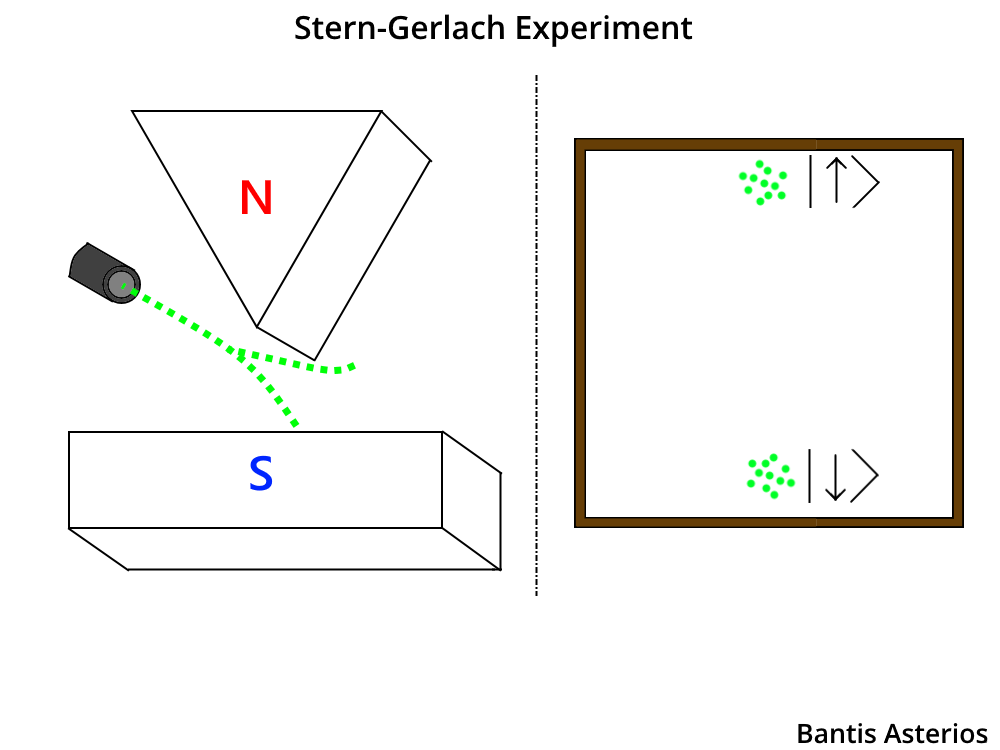
\includegraphics[scale=0.4]{sterngerl.png}
\end{center}

Several practical applications of spin already exist, including Nuclear Magnetic Resonance Spectroscopy (NMR), Electron Spin Resonance Spectroscopy, Magnetic Resonance Imaging (MRI), Hard Drive read/write-heads (Giant Magnetoresistance, Tunnel Magnetoresistance), spintronics (spin-based transistors, Magnetoresistive RAM), anti-ferromagnetic storage media, and more. The electron’s spin plays a vital role in magnetism, and the photon’s spin is related to the polarisation of light.[10][11]


\subsection{Spin and Magnetism}

Spin, even as an inherently quantum-mechanical phenomenon, can be transported and/or used for the processing and storage of information. The theory of magnetism (and its complexity) is a direct result of the spin and orbital motion of particles, and mainly of the electron. All known materials composed of atoms can be divided into five groups, depending on their magnetic response to a DC magnetic field [11]:

\begin{enumerate}
    \item Diamagnetic: In the absence of an external magnetic field, the net magnetization of such a material is zero. All magnetization disappears after the field is removed. The induced magneticity is weak and opposes the direction of the externally-applied magnetic field. The relative magnetic permeability in diamagnetic materials under an external magnetic field is $\mu_{r} \simeq 0.9999$. Magnets weakly repel diamagnetic materials.
    \pagebreak
    \item Paramagnetic: In the absence of an external magnetic field, paramagnetic materials have a small, non-zero net magnetic moment. Under an external magnetic field, the relative magnetic permeability of paramagnetic materials becomes $\mu_{r} \simeq 1.00001$. A magnet will weakly attract paramagnetic materials. Most materials are either paramagnetic or diamagnetic, and thus, it is often assumed that $\mu_{r} \simeq 1$ for both.
    \item Ferromagnetic: In ferromagnetic materials, the induced magnetic moment can remain even after the external field is removed. It is also possible for the magnetic moments to already be aligned before the external magnetic field is applied. In these materials, the relative magnetic permeability usually is $\mu_{r} \gg 1$. Ferromagnetic materials become paramagnetic above a temperature known as the Curie temperature.
    \item Antiferromagnetic: These materials, like ferromagnetic materials, have ordered magnetic moments. However, unlike the above, neighbouring magnetic moments have the same magnitude but the opposite direction.
    \item Ferrimagnetic: These materials are similar to antiferromagnetic materials, but the magnitude of the magnetic moment is larger in one of the directions.[11]
\end{enumerate}
\begin{center}
    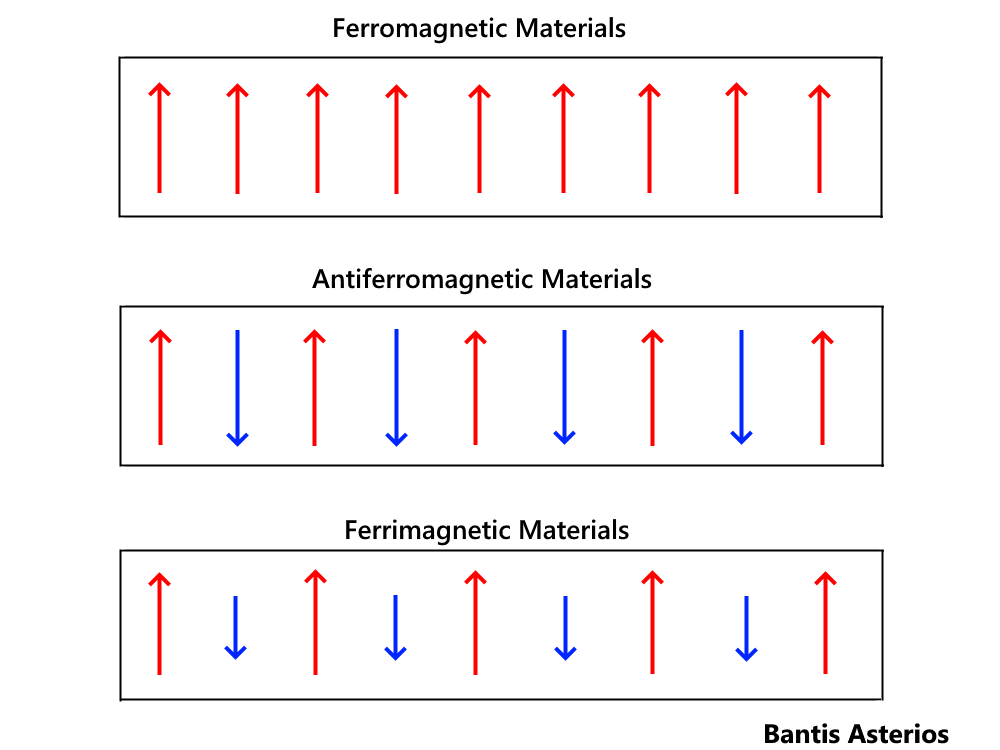
\includegraphics[scale=0.5]{magnetmat.png}
\end{center}

\pagebreak
\section{Introduction to Spintronics}
\subsection{Overview}
Silicon transistors are the key active components in practically all modern electronics and are considered to be one of the greatest inventions of the 20th century.  In contrast to silicon transistors, spin transistors do not actually need electric currents to change their state but utilize the spin of the electrons which is semi-permanent and it can either have the value of spin up (1) or spin down (0). Spin transistors could potentially store more data and use less power than silicon transistors which is very important for the energy demands of the 21st century but no one has actually succeeded in building such a transistor even though the concept was first introduced by Datta and Das at 1990, mostly because of several outstanding technical challenges such as the low spin-injection efficiency due to resistance mismatch, spin relaxation, and the spread of spin precession angle. However, the theory planted the idea that spin could be used in its own right as a means to carry and manipulate information and created the field of 'spintronics'.[14]

\begin{center}
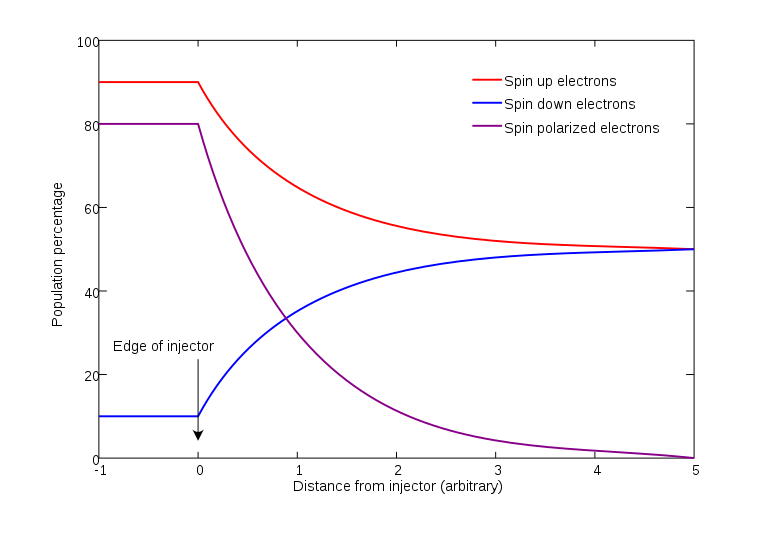
\includegraphics[scale=0.3]{768px-Spin_Injection.svg.png}
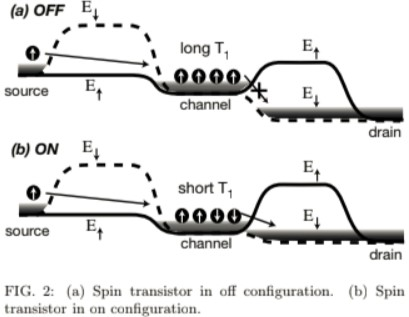
\includegraphics[scale=0.8]{Annotation 2020-10-30 104714.jpg}
\end{center}


\subsection{Spin-transfer Torque}
Spin-transfer torque (STT) is an effect in which the orientation of a magnetic layer in a magnetic tunnel junction or spin valve can be modified using a spin-polarized current. Whereas an ordinary electric current has equal populations of spin-up and spin-down electrons, a spin-polarized current necessarily has unequal populations of electrons. By passing a current through a thick magnetic layer usually called the fixed layer, one can produce a spin-polarized current. If this spin-polarized current is directed into a second, thinner magnetic layer the angular momentum can be transferred to this layer, changing its orientation. This can be used to excite oscillations or even flip the orientation of the magnet. The effects are usually seen only in nanometer-scale devices. STT requires a large spin current passing through a small passageway hence, a preferred geometry is that of the nanopillar. Spin-Transfer Torque effects including nano-oscillators and a novel method of switching Magnetic Tunnel Junctions, enable the scaling of magnetic random access memory (MRAM)  making it possible to create MRAM devices combining low current requirements and reduced cost. However, the amount of current needed to reorient the magnetization is presently too high for most commercial applications, and the reduction of this current density alone is the basis for present academic research in spin electronics.[12]

\begin{center}
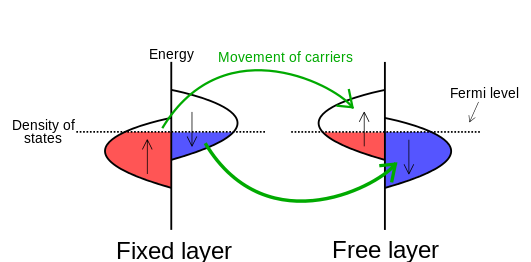
\includegraphics[scale=0.45]{Spin_Transfer_Torque_with_Stoner_model.svg.png}
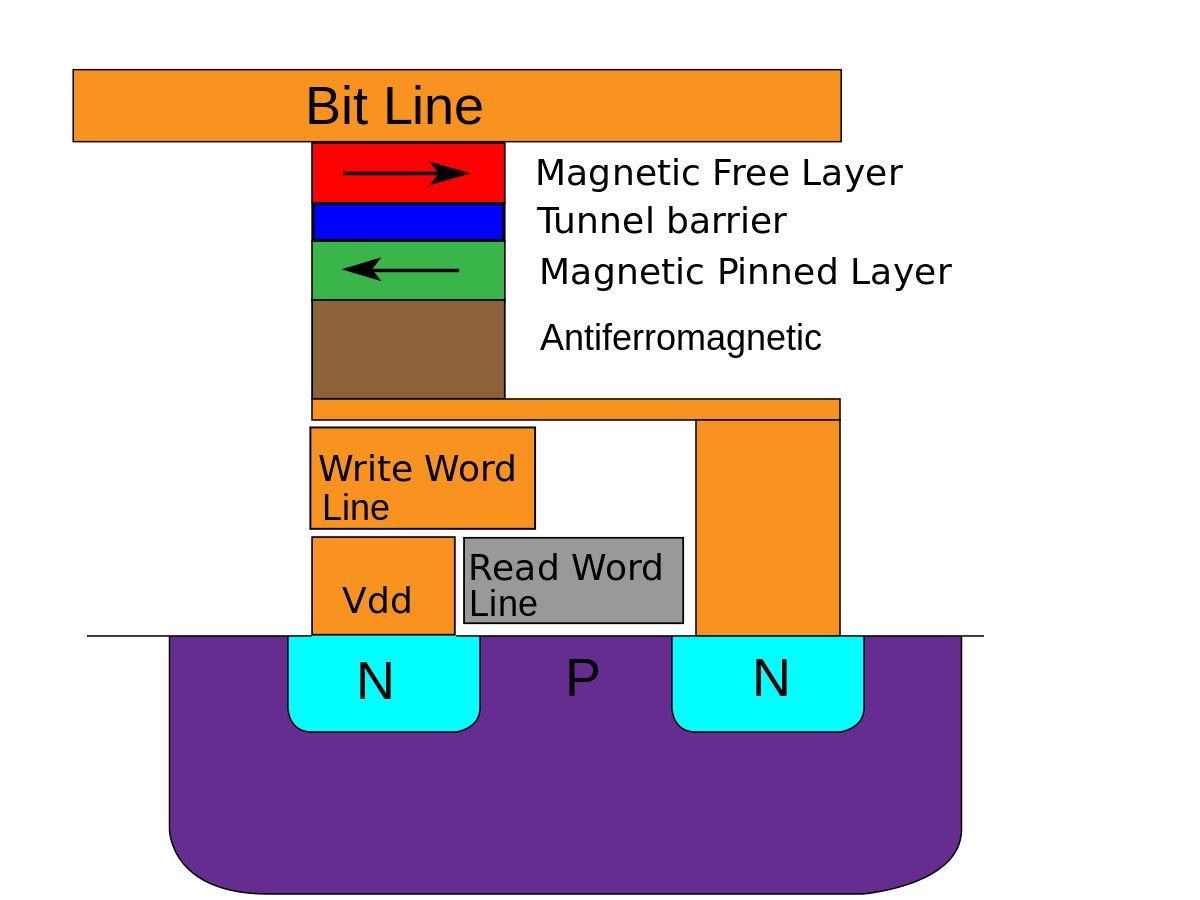
\includegraphics[scale=0.15]{1200px-MRAM-Cell-Simplified.svg.png}
\end{center}

\subsection{Spin Valve}
A device that consists of two or more conducting magnetic materials, whose electrical resistance can change between two values depending on the relative alignment of the magnetization in the layers. The most common applications of this effect involve giant magnetoresistance (GMR) devices. The spin valve acts as a sensor as it flies above the magnetic recording medium, sensing transitions between bits as their stray field reverses.[13]

\begin{center}
    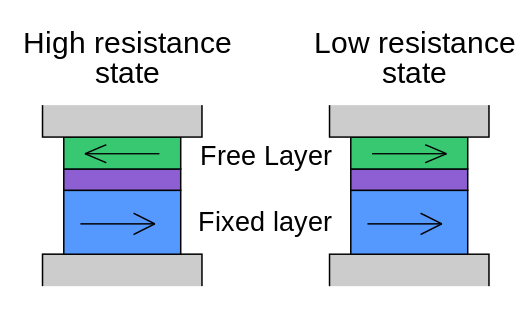
\includegraphics[scale=0.41]{Spin_valve_schematic.svg.png}
    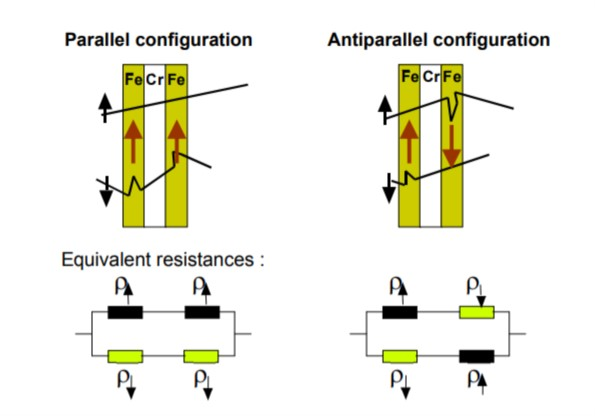
\includegraphics[scale=0.6]{Annotation 2020-10-26 154743.jpg}
\end{center}

\subsection{Giant Magnetoresistance}
A typical GMR device based on the GMR effect for which the Nobel Prize in Physics was awarded in 2007 to Albert Fert and Peter Grunberg has two ferromagnetic layers while between them a nonferromagnetic metal spacer of nanometer thickness. When the magnetizations of the two ferromagnetic layers are parallel, the valve is open or in a low resistance state. When the two are antiparallel, the valve is closed or in a high resistance state. Read heads of magnetic hard drives are based on the GMR or TMR effect.[12][13]

The GMR phenomenon can be described using two spin-related conductivity channels corresponding to the conduction of electrons, for which the resistance is minimum or maximum. The relation between them is often defined in terms of the coefficient of the spin anisotropy β. This coefficient can be defined using the minimum and maximum of the specific electrical resistivity ρF± for the spin-polarized current in the form
$\displaystyle \rho _{F\pm }={\frac {2\rho _{F}}{1\pm \beta }}$, 
where ρF is the average resistivity of the ferromagnet
In magnetically ordered materials, the electrical resistance is crucially affected by scattering of electrons on the magnetic sublattice of the crystal, which is formed by crystallographically equivalent atoms with nonzero magnetic moments. Scattering depends on the relative orientations of the electron spins and those magnetic moments: it is weakest when they are parallel and strongest when they are antiparallel; it is relatively strong in the paramagnetic state, in which the magnetic moments of the atoms have random orientations. In some materials, the interaction between electrons and atoms is the weakest when their magnetic moments are antiparallel rather than parallel. A combination of both types of materials can result in a so-called inverse GMR effect.
Many combinations of materials exhibit GMR, and the most common are the following:

\begin{itemize}
    \item $FeCr$
    \item $Co_{10}Cu_{90}$: $\delta_{h}= 40\%$ at room temperature
    \item $[110]Co_{95}Fe_{5}/Cu$: $\delta_{h} = 110\%$ at room temperature
\end{itemize}

The magnetoresistance depends on many parameters such as the geometry of the device (CIP or CPP), its temperature, and the thicknesses of ferromagnetic and non-magnetic layers.

\begin{center}
    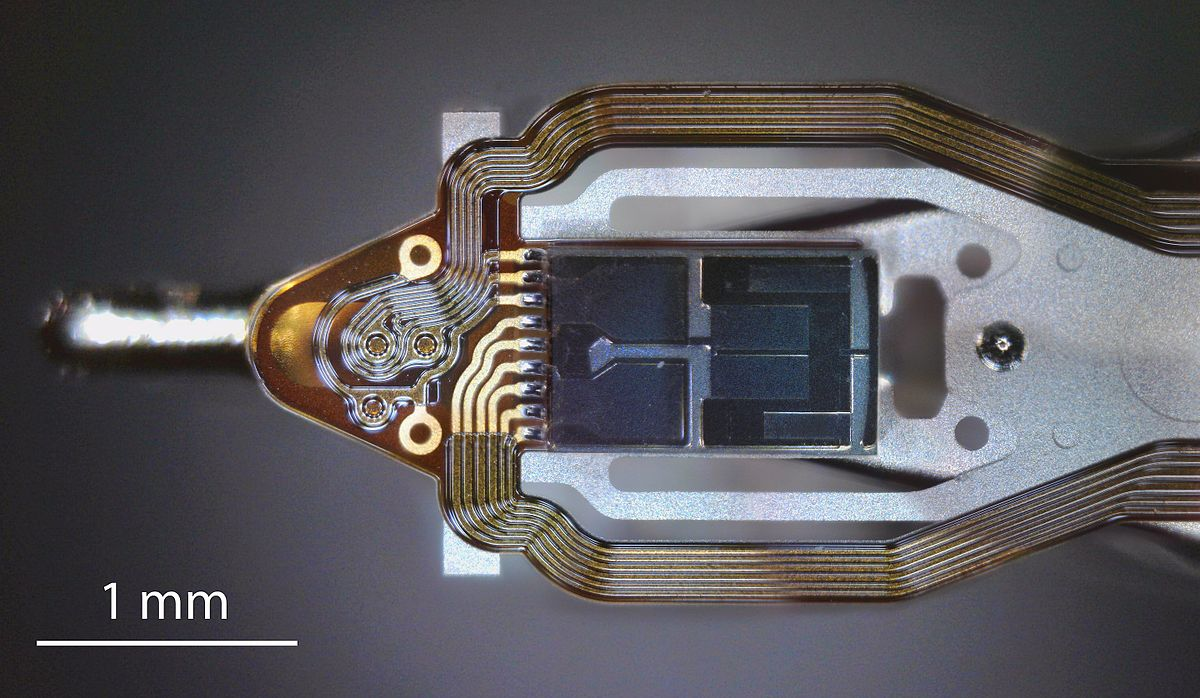
\includegraphics[scale=8]{HDD_read-write_head.jpg}
\end{center}

\subsection{Spin-Orbit Coupling}
 Electrons in atoms can be described by four quantum numbers: energy ($n$), angular momentum ($\ell$), magnetic moment ($m_{\ell}$), and spin ($m_{s}$).[16] The Spin-Orbit Coupling (or Spin-Orbit Effect) is a relativistic quantum-mechanical electromagnetic interaction of an unpaired electron’s angular momentum $\ell$ and spin $m_{s}$, shifting the electron’s energy level, $n$. This phenomenon is often detected with a spectrometer, due to the splitting of spectral curves. This splitting is detectable in any orbital other than the $s$ orbital, which is rotationally/spherically symmetric in every axis.[9][15]

\begin{center}
    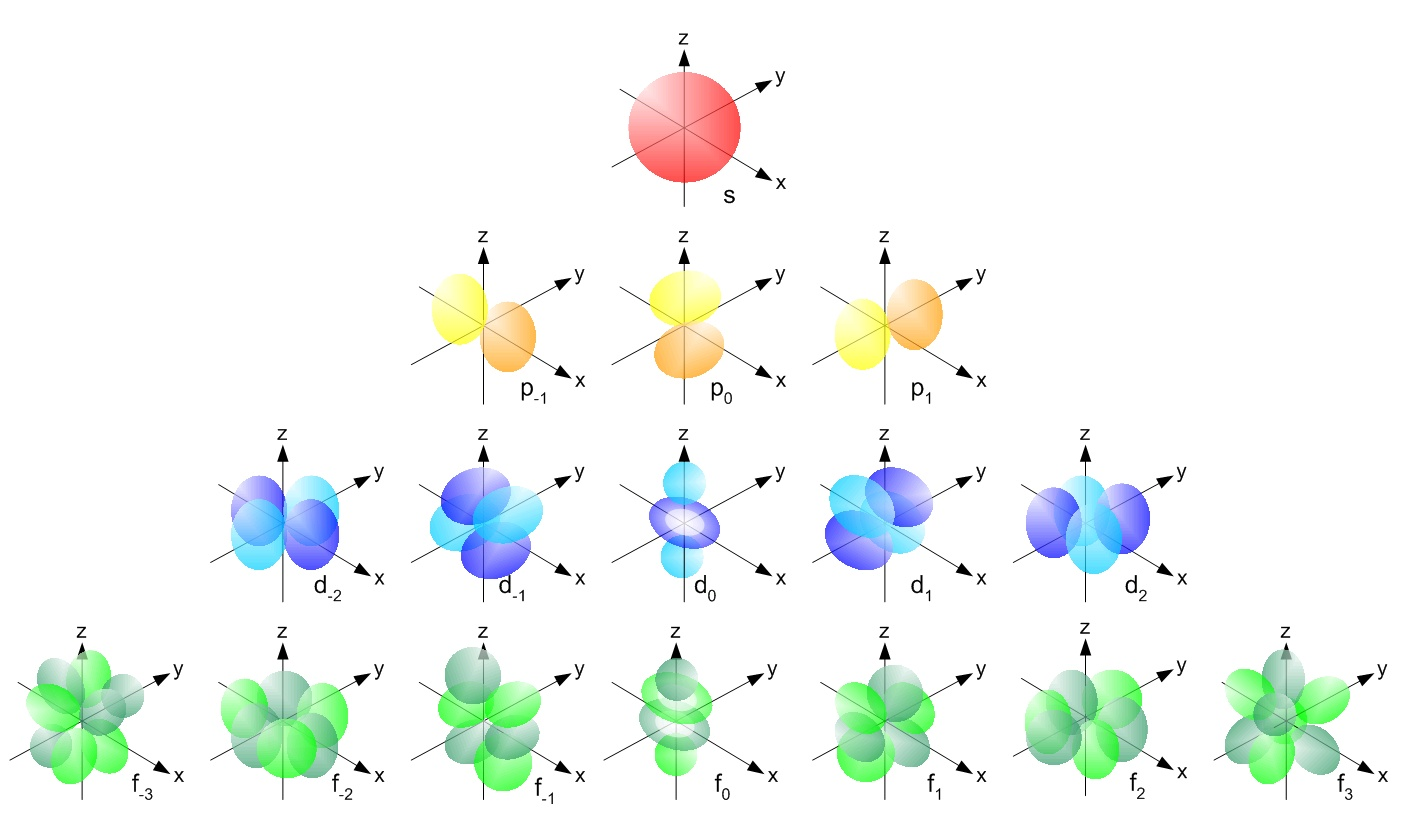
\includegraphics[scale=0.25]{K5EcA.jpg}
\end{center}

The interaction of $\ell$ and $m_{s}$ describes the total angular momentum $J = | \ell + M_{s} |$. Electrons with a different value of $J$ will create different spectral peaks. For an $s$ orbital, $J = | 0 \pm \frac{1}{2} | \Rightarrow J = \frac{1}{2}$, therefore only having a single peak. Similarly for other orbitals, $\ell$ is replaced by the appropriate value. The degeneracy of each state can be calculated with the formula $2J+1=m(j)$.[9][15][17]\\

\subsection{Spin Hall Effect}
Spin Hall Effect: The spin Hall effect is a purely spin-based analogue to the classical Hall effect. Its existence was theorised by the Soviet scientists M. I. Dyakonov and V. I. Perel in 1971.[18] The classical Hall effect, discovered by Edwin Hall in 1879, describes the creation of a voltage difference, $V_{Hall}$, across a conductor, transverse to the direction of the current and to an externally-applied magnetic field, perpendicular to the current.[19][20] Similarly, the spin Hall effect describes the net accumulation of spin on the sides of a conductor, parallel to the direction of the electric current, thus creating a spin voltage/current perpendicular to the electric current, without requiring the presence of a magnetic field. The spin Hall effect is a direct result of spin-orbit interactions.[19][21]

\begin{center}
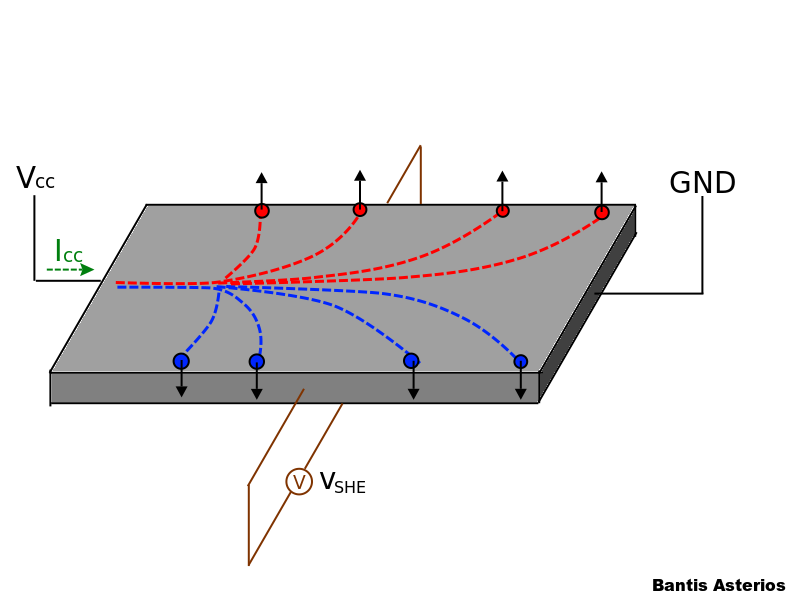
\includegraphics[scale=0.35]{spinhalleffect.png}
\end{center}

The quantum spin Hall state is a state of matter proposed to exist in special, two-dimensional, semiconductors that have a quantized spin-Hall conductance and a vanishing charge-Hall conductance. The quantum spin Hall state of matter is the cousin of the integer quantum Hall state, and that does not require the application of a large magnetic field. In the presence of spin-orbit coupling, certain topological insulators exhibit the QSHS in zero magnetic fields, supporting pure spin-polarized surface edge currents. The first proposal for the existence of a quantum spin Hall state was developed by Charles Kane and Gene Mele who adapted an earlier model for graphene by F. Duncan M. Haldane which exhibits an integer quantum Hall effect. Graphene is such a rich and active field from the point of view of spintronics possesses unique electronic properties, in addition to long spin lifetimes and long spin diffusion lengths. A very important achievement was the realization that the quantum spin Hall state remains to be non-trivial even after the introduction of spin-up and spin-down scattering, which destroys the quantum spin Hall effect.[22][29][30][31][32][33]

\section{Spin Transistors}

\subsection{Spin-Valve Transistor}

The Spin-Valve Transistor (SVT), introduced in 1995, is a device that takes advantage of spintronics and classical transistor mechanics. Like the BJT, it possesses a collector, a base, and an emitter, but unlike the BJT, the Spin Valve Transistor’s base is made of alternating layers of ferromagnetic and non-ferromagnetic metals. Utilizing the Spin Valve effect mentioned in Chapter 3, the ferromagnetic layers work as spin polarizers and spin detectors. In this way, the spin polarization of the base controls the logical state of the electron (high/low). However, the SVT’s $\alpha$, or $\frac{I_{c}}{I_{e}}$ is several orders of magnitude smaller than 1, resulting in a $\beta \ll 1$. Therefore, the Spin Valve Transistor cannot be used as an amplifier or an integrated circuit component. They can be constructed with vacuum metal bonding on Si wafers.[34][35]

\subsection{Bipolar Spin Transistor}
The spin-based equivalent of the Bipolar Junction Transistor (BJT) is the Magnetic Bipolar Transistor (MBT). It uses p-type and n-type ferromagnetic semiconductors for the construction of the pn junctions and has similar properties to its classical counterpart. It utilizes the spin injection mechanism on the emitter, creating a mechanism similar to the Spin Valve effect, making electrons with parallel and antiparallel spin to pass through the junctions with different potentials. The MBT’s $\alpha$ has values close to 1 and the device itself is suitable as an amplifier and an integrated circuit component, albeit facing the same problems as normal BJTs. Furthermore, all III-V-based and IV-based ferromagnetic semiconductors developed so far still have a Curie temperature lower than the human body’s normal temperature. Both MBTs and SVTs are potential-effect transistors.[35][36]

\subsection{Spin-FET}
The Spin-FET, proposed by Datta and Das, consists of an FM source and drain which, respectively, inject and detect the spin-polarized carrier. and uses a fixed ferromagnetic source (S) as a polarizer and a fixed ferromagnetic drain (D) as a detector and exploits the Rashba spin-orbit interaction to determine the spin state the drain will detect. For this purpose, materials with a strong spin-orbit interaction (such as InGaAs and InAs) are placed between the channel and the substrate. The operating principle of the switching operation can be achieved by the spin precession or dephasing of spin-polarised carriers injected in the channel. The substrate and channel are composed of III-V molecules.
The transistor's state depends on whether the electrons' spin state is parallel or antiparallel with the spin direction of the ferromagnetic drain. The magnitude of the Rashba spin-orbit interaction can be controlled by the gate’s (G) voltage. The Spin-FET's performance is limited by the channel length needed to make the injected spin polarization reverse, because the gate can only control the spin-orbit interaction in the transistor's n-channel region.[14][24][35]

\subsection{Spin-MOSFET}

In a Spin-MOSFET, the relative magnetization configurations of the source and drain are used to modify output currents to perform of the "On/Off" operation of the Spin-MOSFET. This operation is based on the gate-bias-induced modification of the Schottky barrier width out of the source/channel junction. Tuning the contact resistance is required for the elimination of the conductivity mismatch problem, high current drivability and high spin injection efficiency. The spin-MOSFET shows great parallel magnetization, and the drain current is highly regulated in antiparallel magnetization. The subthreshold leakage change current of spin-MOSFETs depends on the magnetization configuration of the ferromagnetic source/drain.  The Spin-MOSFET instead uses a silicon substrate and channel and a ferromagnetic source and drain. The spin’s state is determined by the polarization of the ferromagnetic layers.[35][37]


\begin{center}
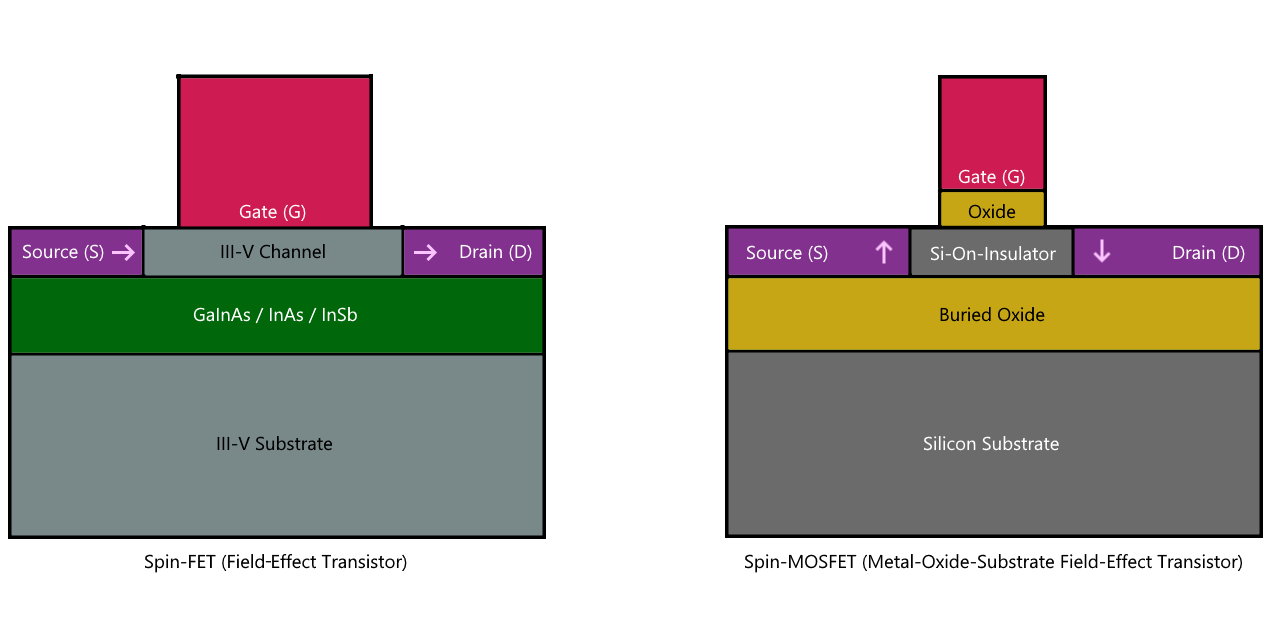
\includegraphics[scale=0.4]{SpinTransistorsBantis.png}
\end{center}

\subsection{Pseudo-Spin MOSFET}
The Pseudo-Spin MOSFET is a pseudo-spintronic device composed of a magnetic tunnel junction and a  “traditional” MOSFET. Connecting a magnetic tunnel junction in series with the MOSFET’s source can reproduce some of the effects of a spin-based transistor. The Magnetic Tunnel Junction supplies the MOSFET with its voltage drop to the source and with negative feedback dependent on its own resistance. The PS-Mosfet can establish magnetic-field-free current-induced magnetization switching for the MJT allowing it to reproduce the spin transistor behaviour being the most advanced transistor on the present MRAM field. Also, the magnetization properties of the MJT can provide high and low current drivability, however, that drivability could be degraded on higher resistance values of the MJT. Therefore, the Pseudo-Spin MOSFET can create a “HIGH” state and a “LOW” state (logical “1” and logical “0”) purely with the electrons’ spin state, even with a constant voltage bias on the MOSFET’s gate. Of all the above candidates, this transistor is the most likely candidate for widespread use in the near future, by applying the technology used in MRAM cells to contemporary MOSFET logic designs, such as PMOS, NMOS, and CMOS. A prototype P-S MOSFET has already been fabricated. The preferable configurations of the PS-MOSFET depend on its area of application with CIM being commonly used to the circuit configuration or with the usage of the difference of drain currents in parallel and antiparallel magnetization configurations.[35]	

\mbox{}
\vfill
\section{Bibliography}
\small
[1] \href{https://journals.aps.org/rmp/abstract/10.1103/RevModPhys.71.S96}{The standard model of particle physics
Mary K. Gaillard, Paul D. Grannis, and Frank J. Sciulli
Rev. Mod. Phys. 71, S96 – Published 1 March 1999}\\[0pt]
[2] \href{https://royalsocietypublishing.org/doi/pdf/10.1098/rspa.1926.0133}{On the Theory of Quantum Mechanics
Paul Adrien Maurice Dirac
Published:01 October 1926}\\[0pt]
[3] \href{https://arxiv.org/abs/cond-mat/9912229}{On the Quantization of the Monoatomic Ideal
Gas
E. Fermi
1926}\\[0pt]
[4] \href{https://books.google.com/books/about/Fundamentals_of_Statistical_and_Thermal.html?id=w5dRAAAAMAAJ&redir_esc=y}{Fundamentals of Statistical and Thermal Physics
Frederick Reif, Reif Federick
McGraw-Hill, 1965 }\\[0pt]
[5] \href{http://www.condmat.uni-oldenburg.de/TeachingSP/bose.ps}{Plancks Gesetz und Lichtquantenhypothese. 
Von Bose
02 July 1924}\\[0pt]
[6] \href{https://archive.org/details/quantummechanics00merz_136/page/n385/mode/2up}{Quantum Mechanics (3rd ed.). pp. 372–3
Merzbacher, Eugen
1998}\\[0pt]
[7]
\href{https://en.wikisource.org/wiki/Relativity:_The_Special_and_General_Theory}{Relativity: The Special and General Theory
Albert Einstein, translation by Robert William Lawson
1916}\\[0pt]
[8] \href{https://www.cup.gr/book/kvantomichaniki-i/}{ Quantum Mechanics I
Stefanos Trachanas
2016 Edition}\\[0pt]
[9] \href{https://archive.org/details/introductiontoqu00grif_190}{Introduction to quantum mechanics
Griffiths, David J.
1942}\\[0pt]
[10] \href{https://www.researchgate.net/publication/260103630_SPINTRONICS_AND_SPINTRONIC_DEVICES}{SPINTRONICS AND SPINTRONIC DEVICES
Vineeth Kartha
November 2011}\\[0pt]
[11] \href{https://books.google.com/books?redir_esc=y&id=L7AUi7ltCksC&focus=searchwithinvolume&q=Spintronics}{Fundamentals of Nanoelectronics
Hanson George W.
2008}\\[0pt]
[12] \href{https://www.springer.com/cn/book/9783642371714}{Giant Magnetoresistance (GMR) Sensors. Smart Sensors, Measurement and Instrumentation
Reig, C., Cardoso, S., \& Mukhopadhyay, S. C.
2013.}\\[0pt]
[13] \href{https://pubmed.ncbi.nlm.nih.gov/17972936/}{The emergence of spin electronics in data storage
Chappert, C., Fert, A., \& Van Dau, F. N. 
2007}\\[0pt]
[14] \href{https://aip.scitation.org/doi/10.1063/1.102730}{Electronic analog of the electro‐optic modulator
Datta, S., \& Das, B. 
1990}\\[0pt]
[15] \href{https://arxiv.org/pdf/cond-mat/0408119.pdf}{Spin Dynamics and Spin Transport
Emmanuel I. Rashba
2004}\\[0pt]
[16] \href{http://ebooks.edu.gr/ebooks/handle/8547/2359}{Χημεία Κατεύθυνσης, Γ’ Γενικού Λυκείου
Hellenic Ministry of Education, Research, and Religious Affairs
2015}\\[0pt]
[17] \href{https://www.sciencedirect.com/science/article/abs/pii/S0921452602011109?via\%3Dihub}{Crystal-field interactions and magnetism in rare-earth transition-metal intermetallic compounds
R. J. Radwanski, R. Michalski, Z. Ropka, A. Blaut
2002}\\[0pt]
[18] \href{http://www.jetpletters.ac.ru/cgi-bin/articles/download.cgi/1587/article_24366.pdf}{Possibility of Orienting Electron Spins with Current
Dyakonov M.I., Perel V. I.
1971}\\[0pt]
[19] \href{https://web.archive.org/web/20110727010116/http://www.stenomuseet.dk/skoletj/elmag/kilde9.html}{On a New Action of the Magnet on Electric Currents
E. H. Hall
1879}\\[0pt]
[20] \href{https://www.britannica.com/science/Hall-effect}{Encyclopedia Britannica: Hall effect}\\[0pt]
[21] \href{https://journals.aps.org/prl/abstract/10.1103/PhysRevLett.83.1834}{Spin Hall Effect
J. E. Hirsch
1999}
[22] \href{https://www.annualreviews.org/doi/full/10.1146/annurev-conmatphys-070909-104123}{Annual Review of Condensed Matter Physics, Vol. 1,
S.D. Bader, S.S.P. Parkin
2010}\\[0pt]
[23] \href{http://www.ijsrp.org/research-paper-0613.php?rp=P181346}{Utilization of Spintronics, IJSRP, Volume 3, Issue 6
Jitendra S. Pingale, Mukesh D. Patil, Umar I. Masumdar 
June 2013}\\[0pt]
[24] \href{https://aip.scitation.org/doi/10.1063/1.2192152}{Performance of a spin-based insulated gate field effect transistor
Kimberley C. Hall, Michael E. Flatte
2016}\\[0pt]
[25] Concise encyclopedia of magnetic and superconducting materials (2nd ed.)
Buschow, K. H. J.
2005\\[0pt]
[26] Physical foundations of spin electronics
Tretyak, O. V.; Lvov, V. A.; Barabanov, O. V.
2002\\[0pt]
[27] \href{https://web.archive.org/web/20110724184833/http://web.phys.tue.nl/fileadmin/tn/de_faculteit/capaciteitsgroepen/FM/FNA/Students_Education/Lectures_Courses/Coehoorn_Lecture-Notes-SVs-Part1-final.pdf}{Novel Magnetoelectronic Materials and Devices.
Coehoorn, R.
2003}\\[0pt]
[28] \href{https://journals.aps.org/prb/pdf/10.1103/PhysRevB.39.4828}{Enhanced magnetoresistance in layered magnetic structures with antiferromagnetic interlayer exchange
Binasch, G.; Grunberg; Saurenbach; Zinn
1989}\\[0pt]
[29] \href{https://arxiv.org/abs/cond-mat/0411737}{Quantum Spin Hall Effect in Graphene
Kane, C.L.; Mele, E.J.
25 November 2005}\\[0pt]
[30] \href{http://eprints.whiterose.ac.uk/158329/1/1_s2.0_S0304885320302353_main.pdf}{Review on spintronics: Principles and device applications: Atsufumi Hirohataa, Keisuke Yamadab, Yoshinobu Nakatanic, Ioan-Lucian Prejbeanud, Bernard Diényd, Philipp Pirro, Burkard Hillebrandse
2020}\\[0pt]
[31] \href{https://journals.aps.org/prl/abstract/10.1103/PhysRevLett.96.106802}{Quantum Spin Hall Effect". Physical Review Letters. 96
Bernevig, B. Andrei; Zhang, Shou-Cheng
14 March 2006}\\[0pt]
[32] \href{https://journals.aps.org/prl/abstract/10.1103/PhysRevLett.95.146802}{Z2 Topological Order and the Quantum Spin Hall Effect, Physical Review Letters. 95
Kane, C.L.; Mele, E.J
28 September 2005}\\[0pt]
[33] \href{https://science.sciencemag.org/content/318/5851/766}{"Quantum Spin Hall Insulator State in HgTe Quantum Wells". Science. 318
König, Markus; Wiedmann, Steffen; Brüne, Christoph; Roth, Andreas; Buhmann, Hartmut; Molenkamp, Laurens W.; Qi, Xiao-Liang; Zhang, Shou-Cheng
November 2, 2007}\\[0pt]
[34] Jansen, R. (2003). The spin-valve transistor: a review and outlook. Journal of Physics D: Applied Physics, 36(19), R289–R308.\\[0pt]
[35] Sugahara, S., \& Nitta, J. (2010). Spin-Transistor Electronics: An Overview and Outlook. Proceedings of the IEEE, 98(12), 2124–2154. \\[0pt]
[36] Fabian, J., Žutić, I., \& Das Sarma, S. (2004). Magnetic bipolar transistor. Applied Physics Letters, 84(1), 85–87.\\[0pt]
[37] \href{https://aip.scitation.org/doi/10.1063/1.1689403}{A spin metal-oxide-semiconductor field-effect transistor using
half-metallic-ferromagnet contacts for the source and drain
S. Sugahara, M. Tanaka
2004}

\end{document}
